% SIWAT classification engine (spec v2.0, section 5): condition -> light -> law -> channels.
\documentclass[border=12pt]{standalone}
\usepackage{tikz}
\usetikzlibrary{arrows.meta,positioning,calc,shapes.geometric}
\definecolor{siwatPlum}{HTML}{38113B}
\definecolor{siwatRed}{HTML}{E63946}
\definecolor{siwatRedText}{HTML}{A61B29}
\definecolor{siwatYellow}{HTML}{C99A1E}
\definecolor{siwatYellowText}{HTML}{6E5100}
\definecolor{siwatGreen}{HTML}{2A9D8F}
\definecolor{siwatGreenText}{HTML}{1B6B61}
\definecolor{siwatEdge}{HTML}{DDD1DA}
\definecolor{siwatMuted}{HTML}{63506A}
\renewcommand{\familydefault}{\sfdefault}
\hyphenpenalty=10000 \exhyphenpenalty=10000
\begin{document}
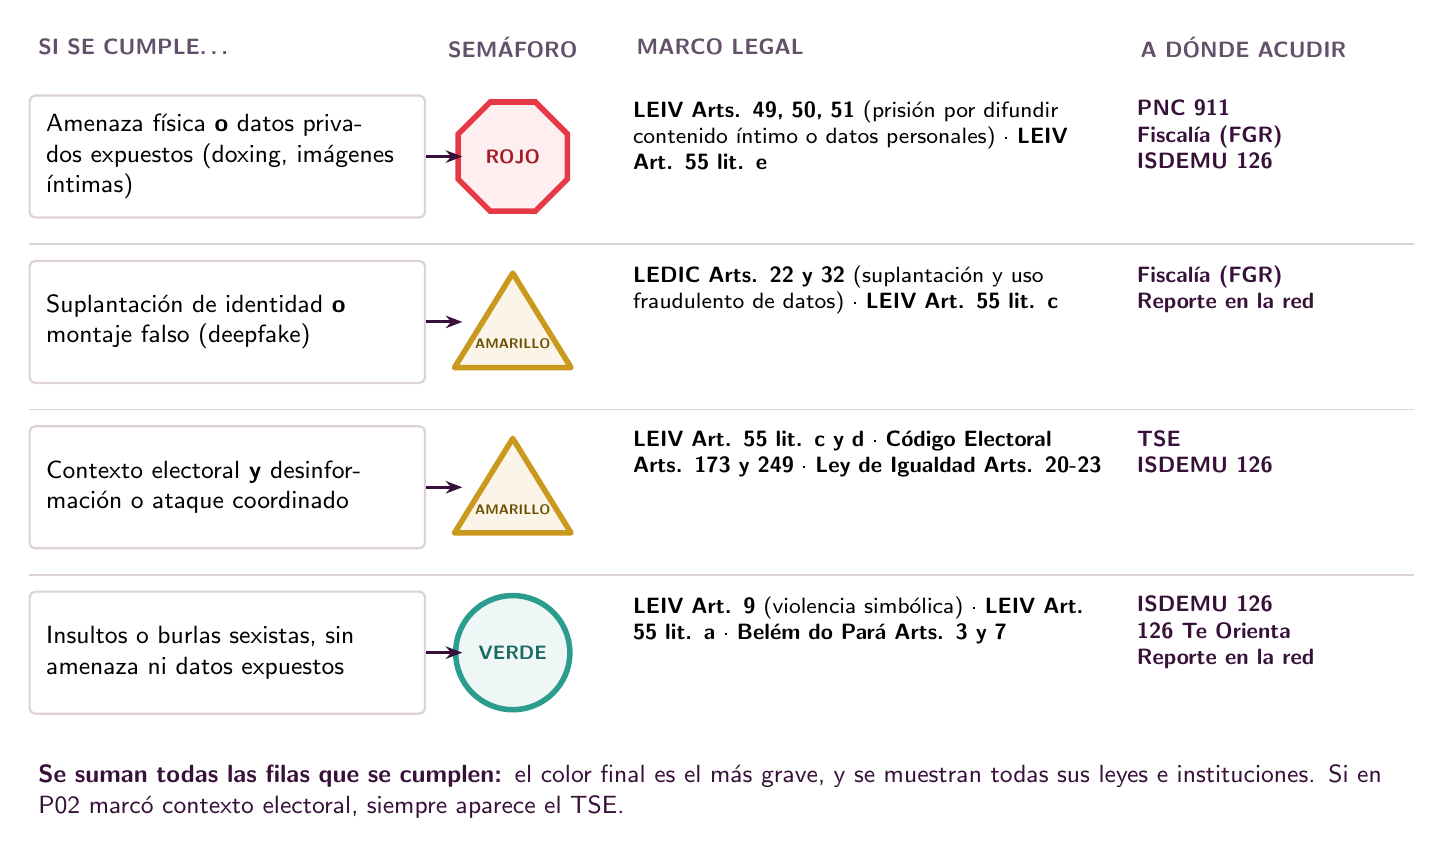
\begin{tikzpicture}[
  font=\sffamily,
  >={Stealth[length=6pt]},
  cond/.style={draw=siwatEdge, line width=0.8pt, fill=white, rounded corners=2pt, text width=4.6cm,
    minimum height=1.55cm, align=left, font=\small, inner sep=6pt},
  law/.style={text width=6.0cm, align=left, font=\footnotesize, inner sep=2pt},
  inst/.style={text width=3.5cm, align=left, font=\footnotesize\bfseries, text=siwatPlum, inner sep=2pt},
  head/.style={font=\footnotesize\bfseries, text=siwatMuted},
  link/.style={->, line width=1.1pt, draw=siwatPlum},
]
% Column heads
\node[head, anchor=west] at (0,0.9) {SI SE CUMPLE\ldots};
\node[head] at (6.15,0.9) {SEMÁFORO};
\node[head, anchor=west] at (7.6,0.9) {MARCO LEGAL};
\node[head, anchor=west] at (14.0,0.9) {A DÓNDE ACUDIR};

% Rows: y positions
\def\rowA{0} \def\rowB{-2.1} \def\rowC{-4.2} \def\rowD{-6.3}

% Row A: red
\node[cond, anchor=north west] (ca) at (0,\rowA+0.3) {Amenaza física \textbf{o} datos privados expuestos (doxing, imágenes íntimas)};
\node[regular polygon, regular polygon sides=8, draw=siwatRed, line width=2pt, fill=siwatRed!8,
  minimum size=1.5cm, font=\scriptsize\bfseries, text=siwatRedText] (la) at (ca.center -| 6.15,0) {ROJO};
\node[law, anchor=north west] at (7.6,\rowA+0.3) {\textbf{LEIV Arts. 49, 50, 51} (prisión por difundir contenido íntimo o datos personales) · \textbf{LEIV Art. 55 lit. e}};
\node[inst, anchor=north west] at (14.0,\rowA+0.3) {PNC 911\\Fiscalía (FGR)\\ISDEMU 126};

% Row B: yellow (identity)
\node[cond, anchor=north west] (cb) at (0,\rowB+0.3) {Suplantación de identidad \textbf{o} montaje falso (deepfake)};
\coordinate (lb) at (cb.center -| 6.15,0);
\draw[siwatYellow, line width=2pt, fill=siwatYellow!10, line join=round] ($(lb)+(0,0.62)$) -- ($(lb)+(0.74,-0.58)$) -- ($(lb)+(-0.74,-0.58)$) -- cycle;
\node[font=\tiny\bfseries, text=siwatYellowText] at ($(lb)+(0,-0.28)$) {AMARILLO};
\node[law, anchor=north west] at (7.6,\rowB+0.3) {\textbf{LEDIC Arts. 22 y 32} (suplantación y uso fraudulento de datos) · \textbf{LEIV Art. 55 lit. c}};
\node[inst, anchor=north west] at (14.0,\rowB+0.3) {Fiscalía (FGR)\\Reporte en la red};

% Row C: yellow (electoral)
\node[cond, anchor=north west] (cc) at (0,\rowC+0.3) {Contexto electoral \textbf{y} desinformación o ataque coordinado};
\coordinate (lc) at (cc.center -| 6.15,0);
\draw[siwatYellow, line width=2pt, fill=siwatYellow!10, line join=round] ($(lc)+(0,0.62)$) -- ($(lc)+(0.74,-0.58)$) -- ($(lc)+(-0.74,-0.58)$) -- cycle;
\node[font=\tiny\bfseries, text=siwatYellowText] at ($(lc)+(0,-0.28)$) {AMARILLO};
\node[law, anchor=north west] at (7.6,\rowC+0.3) {\textbf{LEIV Art. 55 lit. c y d} · \textbf{Código Electoral Arts. 173 y 249} · \textbf{\mbox{Ley de Igualdad Arts. 20-23}}};
\node[inst, anchor=north west] at (14.0,\rowC+0.3) {TSE\\ISDEMU 126};

% Row D: green
\node[cond, anchor=north west] (cd) at (0,\rowD+0.3) {Insultos o burlas sexistas, sin amenaza ni datos expuestos};
\node[circle, draw=siwatGreen, line width=2pt, fill=siwatGreen!8, minimum size=1.45cm,
  font=\scriptsize\bfseries, text=siwatGreenText] (ld) at (cd.center -| 6.15,0) {VERDE};
\node[law, anchor=north west] at (7.6,\rowD+0.3) {\textbf{LEIV Art. 9} (violencia simbólica) · \textbf{LEIV Art. 55 lit. a} · \textbf{Belém do Pará Arts. 3 y 7}};
\node[inst, anchor=north west] at (14.0,\rowD+0.3) {ISDEMU 126\\126 Te Orienta\\Reporte en la red};

\foreach \c in {ca, cb, cc, cd} \draw[link] (\c.east) -- ++(0.46,0);

% Row separators
\foreach \y in {-1.6,-3.7,-5.8} \draw[siwatEdge, line width=0.6pt] (0,\y) -- (17.6,\y);

% Combination rule
\node[anchor=north west, text width=17.4cm, font=\small, text=siwatPlum, align=left] at (0,-8.1)
  {\textbf{Se suman todas las filas que se cumplen:} el color final es el más grave, y se muestran todas sus leyes e instituciones. Si en P02 marcó contexto electoral, siempre aparece el TSE.};
\end{tikzpicture}
\end{document}
